\chapter{Supervised learning}
\label{ch:supervised}

Consider a collection of fresh basalt samples originating from
different tectonic settings (e.g., mid ocean ridges, ocean islands and
island arcs).  Suppose that we have analysed the chemical composition
of these samples (i.e., the concentration of SiO\textsubscript{2},
Al\textsubscript{2}O\textsubscript{3}, etc). Further suppose that we
have also analysed a basaltic rock from an ophiolite of unknown
origin.  Can we recover the original tectonic setting of the
ophiolite?\\

This is one example of a supervised learning problem. Whereas the
unsupervised learning algorithms of chapter~\ref{ch:unsupervised} do
not require prior knowledge about the data, the supervised learning
algorithms of this chapter use \textbf{training data} to classify
samples into pre-defined categories. Once the classification is
complete, the same decision rules can then be used to assign a new
sample of unknown affinity to one of these categories.\\

This chapter will introduce two supervised learning techniques.
Discriminant analysis (Section~\ref{sec:LDA}) is a method that is
similar in some ways to PCA (Section~\ref{sec:PCA}), whereas decision
trees (Section~\ref{sec:CART}) are similar in some ways to the
hierarchical clustering algorithm of Section~\ref{sec:hierarchical}.

\section{Discriminant Analysis}
\label{sec:LDA}

Consider a dataset $X$ containing a large number of $N$-dimensional
data, which belong to one of $K$ classes. We are trying to decide
which of these classes an unknown sample $x$ belongs to.  This
question is answered by Bayes' Rule
(Section~\ref{sec:conditionalprobability}): the decision $d$ is the
class $G$ ($1 \leq G \leq K$) that has the highest \textbf{posterior
  probability} given the data $x$:
\begin{equation}
  \label{eq:bayesRule}
  d = \underset{k=1,\ldots,K}{\max} P(G=k|X=x)
\end{equation}

This posterior probability can be calculated using Bayes' Theorem
(Equation~\ref{eq:Bayes}):
\begin{equation}
  \label{eq:bayesTheorem}
  P(G|X) \propto P(X|G)P(G)
\end{equation}

\noindent where $P(X|G)$ is the \textbf{likelihood} of the data in a
given class and $P(G)$ the \textbf{prior probability} of the class,
which we will assume to be uniform; i.e.,
$P(G=1)=P(G=2)=\ldots=P(G=K)=1/K$.  Therefore, plugging
Equation~\ref{eq:bayesTheorem} into Equation~\ref{eq:bayesRule}
reduces Bayes' Rule to a comparison of likelihoods.  We now make the
simplifying assumption of multivariate normality:
\begin{equation}
  \label{eq:multiNorm}
  P(X=x|G=k) = \frac{\exp \left[ -\frac{1}{2}(x-\mu_k)^T\Sigma_k^{-1}(x-\mu_k) \right]}{\sqrt{(2\pi)^N|\Sigma_k|}}
\end{equation}

\noindent where $\mu_k$ and $\Sigma_k$ are the mean and covariance of
the $k$\textsuperscript{th} class and $(x-\mu_k)^T$ indicates the
transpose of the matrix ($x-\mu_k$).  Using
Equation~\ref{eq:multiNorm} and taking logarithms,
Equation~\ref{eq:bayesRule} becomes:
\begin{equation}
  \label{eq:quadRule}
  d = \underset{k=1,\ldots,K}{\max}
  \left[-\frac{1}{2}\ln|\Sigma_k| -
    \frac{1}{2}(x-\mu_k)^T\Sigma_k^{-1}(x-\mu_k)\right]
\end{equation}

Equation~\ref{eq:quadRule} forms the basis for \textbf{quadratic
  discriminant analysis} (QDA). Let us illustrate this procedure with
a simple bivariate dataset comprising three classes:\\

\noindent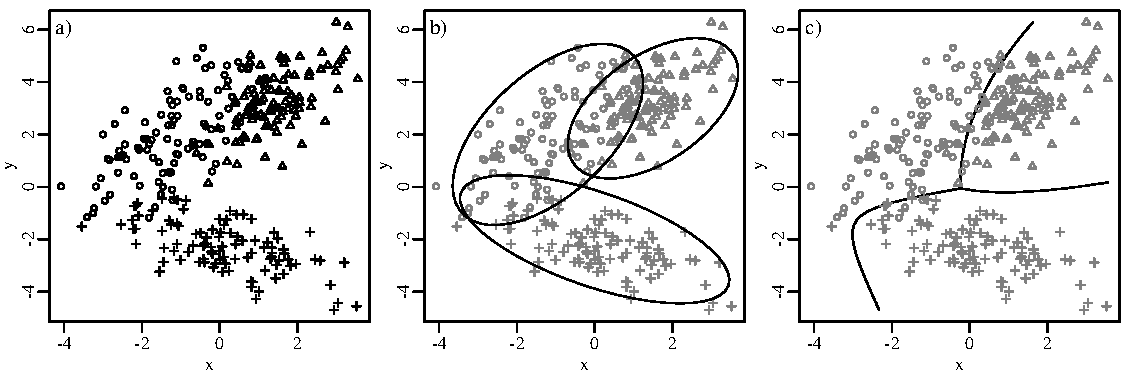
\includegraphics[width=\linewidth]{../figures/QDA.pdf}
\begingroup \captionof{figure}{Quadratic discriminant analysis of
  synthetic data: a) the bivariate training data comprise three
  classes that are marked by crosses, circles and triangles,
  respectively; b) fitting three bivariate normal distributions to the
  data produces c) curved decision boundaries between the three
  distributions.\\}
\label{fig:QDA}\endgroup

If we have a new sample of unknown affinity, then we can simply plot
its $(x,y)$-composition on Figure~\ref{fig:QDA}.c) and classify it in
one of the three groups depending on the decision boundaries.\\

Usually, $\mu_k$ and $\Sigma_k$ are not known, and must be estimated
from the training data.  If we make the additional assumption that all
the classes share the same covariance structure (i.e., $\Sigma_k =
\Sigma$ for all $k$), then Equation~\ref{eq:bayesRule} simplifies to:
\begin{equation}
  \label{eq:linRule}
d = \underset{k=1,\ldots,K}{\max}\left[
x^T\Sigma^{-1}\mu_k-\frac{1}{2}\mu_k^T\Sigma^{-1}\mu_k \right]
\end{equation}

This is the basis of \textbf{linear discriminant analysis} (LDA),
which has some desirable properties.  Because
Equation~\ref{eq:linRule} is linear in $x$, the decision boundaries
between the different classes are straight lines. Figure~\ref{fig:LDA}
illustrates this phenomenon with a second bivariate dataset:\\

\noindent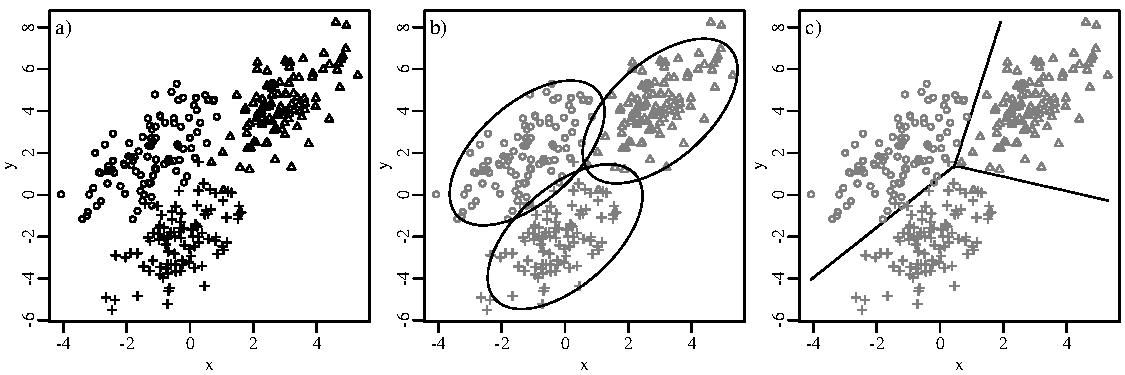
\includegraphics[width=\linewidth]{../figures/LDA.pdf}
\begingroup \captionof{figure}{Linear discriminant analysis of a
  second synthetic dataset: a) the bivariate training data comprise
  the same three classes as Figure~\ref{fig:QDA}; b) fitting three
  bivariate normal distributions to the data with the same covariance
  matrix c) produces linear decision boundaries between the three
  distributions.\\}
\label{fig:LDA}
\endgroup

LDA can also be used to reduce the dimensionality of a dataset, in a
similar way to PCA. Recall that, in Section~\ref{sec:PCA}, we used a
simple toy example to show how PCA can be used to project a
two-dimensional dataset onto a one dimensional line. We can use the
same approach to illustrate how LDA can achieve the same effect with a
different aim. Consider a mixed dataset of two bivariate normal
distributions:\\

\noindent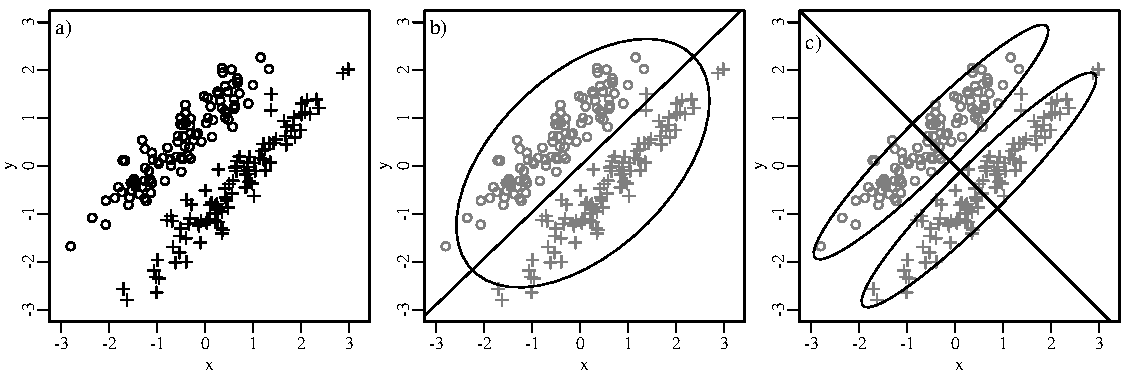
\includegraphics[width=\linewidth]{../figures/PCAvsLDA.pdf}
\begingroup \captionof{figure}{a) an equal mixture of two bivariate
  normal datasets; b) PCA extracts the major axis of the best fitting
  error ellipse to the merged dataset as the first principal
  component; c) LDA fits two error ellipses to the data and extracts a
  function (the first linear discriminant) that maximises the distance
  between them. In this example, this produces a line that is
  perpendicular to the first principal component.\\}
\label{fig:PCAvsLDA}
\endgroup

Applying LDA to the four-dimensional iris dataset produces four linear
discriminant functions that maximise the \textit{between class}
variance (i.e., the variance of the class means) relative to the
\textit{within class} variance (i.e., the pooled variance of the
groups about their means). Like the first two principal components of
Figure~\ref{fig:USArrests} and the first two MDS dimensions of
Figure~\ref{fig:eurodist}, also the first two linear discriminant
function of Figure~\ref{fig:LDAiris} achieve a dimension
reduction. But whereas PCA and MDS aim to visualise the total
variability of the dataset, LDA aims to highlight the pre-defined
clusters within the dataset:

\noindent\begin{minipage}[t][][b]{.35\textwidth}
  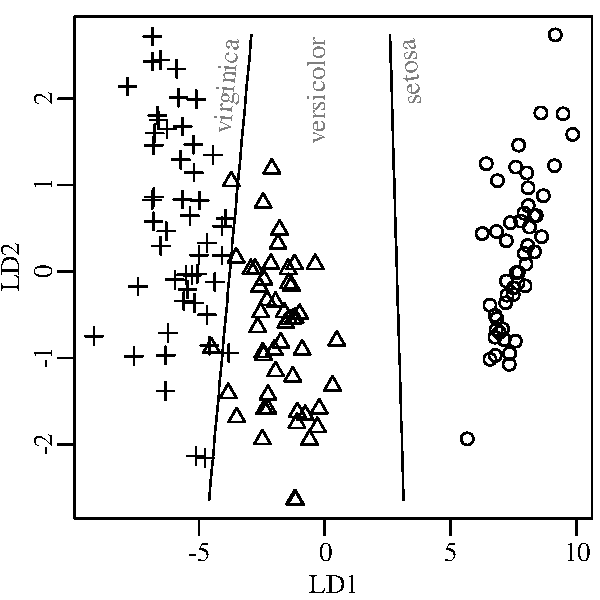
\includegraphics[width=\textwidth]{../figures/LDAiris.pdf}\\
\end{minipage}
\begin{minipage}[t][][t]{.65\textwidth}
  \captionof{figure}{The first two linear discriminants of the
    four-dimensional iris data represent a two-dimensional projection
    of these data that maximises the differences between the three
    different species of flowers. They are defined as\\
    LD1 = 0.83 $\times$ (sepal length - 5.84) + 1.53 $\times$ (sepal width -
    3.06) - 2.20 $\times$ (petal length - 3.76) - 2.81 $\times$ (petal
    width - 1.20); and\\
    LD2 = 0.024 $\times$ (sepal length - 5.85) +
    2.16 $\times$ (sepal width - 3.06) - 0.93 $\times$ (petal length -
    3.76) + 2.84 $\times$ (petal width - 1.20).\\}
  \label{fig:LDAiris}
\end{minipage}

Suppose that we have a new flower with a sepal length of 6.0~cm, a
sepal width of 3.0~cm, a petal length of 5.0~cm and a petal width of
1.5~cm. What species does the flower belong to?

\noindent\begin{minipage}[t][][b]{.35\textwidth}
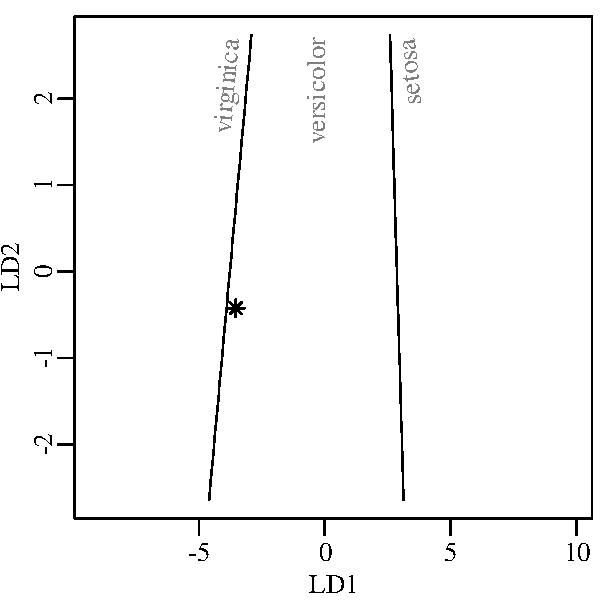
\includegraphics[width=\textwidth]{../figures/LDAnewiris.pdf}\\
\end{minipage}
\begin{minipage}[t][][t]{.65\textwidth}
  \captionof{figure}{ Using the two discriminant functions of
    Figure~\ref{fig:LDAiris}:\\
    LD1 =
    $0.83\times(6.0-5.84)+1.53\times(3.0-3.06)-2.20\times(5.0-3.76)-2.81\times(1.5-1.20)=-3.53$; and\\
    LD2 =
    $0.024\times(6.0-5.85)+2.16\times(3.0-3.06)-0.93\times(5.0-3.76)+2.84\times(1.5-1.20)=-0.42$.\\ Plotting these two coordinates on the discrimination diagram of
    Figure~\ref{fig:LDAiris} suggests that the new flower belongs to
    the \textit{versicolor} species.  \\}
  \label{fig:LDAnewiris}
\end{minipage}

A more precise classification can be obtained by plugging the
measurements of the new flower into Equation~\ref{eq:bayesTheorem} and
calculating the posterior probabilities for the three species.  This
produces the following result:

\begin{center}
\begin{tabular}{cccc}
  & \emph{virginica} & \emph{versicolor} & \emph{setosa} \\ \hline
$P(G|X)$ & 0.19 & 0.81 & $3.2\times{10}^{-27}$
\end{tabular}
\end{center}

In conclusion, there is an 81\% chance that the new flower is
\emph{versicolor} and a 19\% chance that it is \emph{virginica}.

\section{Decision trees}
\label{sec:CART}

Discriminant analysis is a \textit{parametric} learning algorithm,
which assumes that the different classes in a dataset are grouped in
multivariate normal clusters (Figures~\ref{fig:QDA}.b and
\ref{fig:LDA}.b). Here is an example of a dataset for which this
assumption is invalid:

\noindent\begin{minipage}[t][][b]{.35\textwidth}
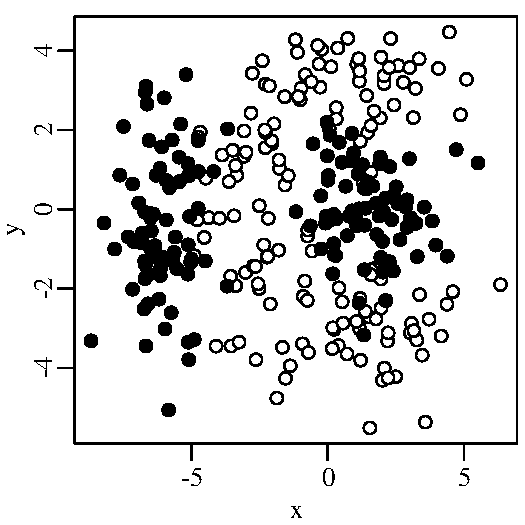
\includegraphics[width=\textwidth]{../figures/CARTdata.pdf}\\
\end{minipage}
\begin{minipage}[t][][t]{.65\textwidth}
  \captionof{figure}{Synthetic dataset of bivariate measurements that
    belong to two classes. The black circles are split into two data
    clouds. The white circles form a `c'-shape surrounding one of the
    modes of the black population. Discriminant analysis is unable to
    deal with this situation.\\}
  \label{fig:CARTdata}
\end{minipage}

Decision trees are a \textit{nonparametric} learning algorithm that is
better able to handle complex multimodal datasets like this. It uses
\textbf{recursive binary partitions} to describe the data, with a
piecewise constant function. The first step of the algorithm
exhaustively searches all the possible split points $s$ ($-\infty < s
< \infty$) and variables ($x$ and $y$ in our example) to minimise the
\textbf{impurity} $Q$:

\begin{equation}
  Q = p_{\circ} (1-p_{\circ}) + p_{\bullet} (1-p_{\bullet})
  \label{eq:Q}
\end{equation}

\noindent where $p_{\circ}$ and $p_{\bullet}$ are the proportions of
class~1 and class~2 objects in one half of the partition.
Equation~\ref{eq:Q} is also known as the \textbf{Gini index} of
diversity.  Figure~\ref{fig:Qtries} evaluates a few possible split
points using this criterion.  The optimal solution is found by
exhaustive searching:\\

\noindent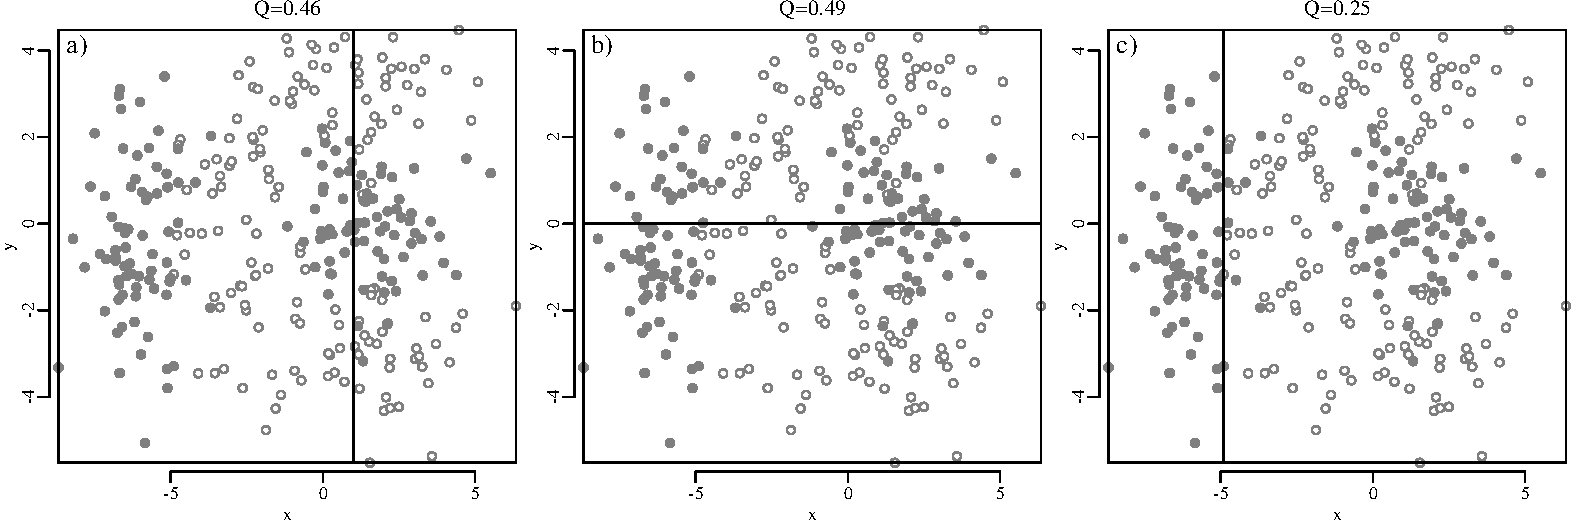
\includegraphics[width=\textwidth]{../figures/Qtries.pdf}
\begingroup \captionof{figure}{Evaluation of three candidate split
  points using the Gini index $Q$. The best first order split
  corresponds to $x=-4.902$ (panel c).\\}
\label{fig:Qtries}
\endgroup

The left hand side of the first partition ($x<-4.902$,
Figure~\ref{fig:Qtries}.c) is pure (100\% $\times\bullet$). So the
second step only needs to evaluate the right hand side. One major
advantage of using \textit{recursive} partitions is that they can be
visualised as dendrograms, just like the hierarchical clusters of
Section~\ref{sec:hierarchical}:\\

\noindent\begin{minipage}[t][][b]{.7\textwidth}
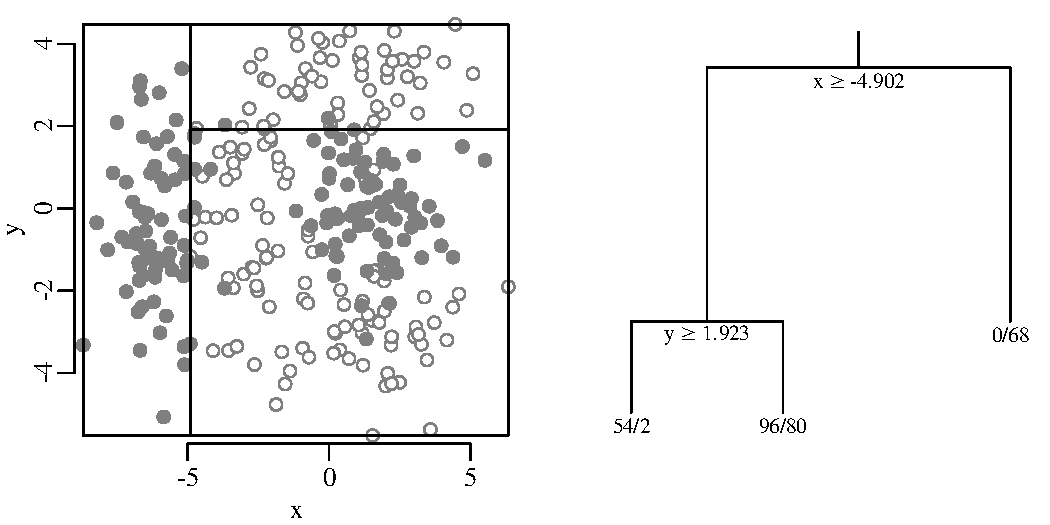
\includegraphics[width=\textwidth]{../figures/Q2.pdf}\\
\end{minipage}
\begin{minipage}[t][][t]{.3\textwidth}
  \captionof{figure}{Second order partition of the right hand side of
    Figure~\ref{fig:Qtries}.c). The results can be visualised as a
    dendrogram or tree (right). The `leaves' of this tree are
    annotated as $n_\circ/n_\bullet$ where $n_\circ$ is the number of
    training data of class $\circ$ and $n_\bullet$ is the number of
    training data of class $\bullet$.\\}
  \label{fig:Q2}
\end{minipage}

The recursive partitioning process can be repeated until all the nodes
of the decision tree are `pure', i.e. they contain only $\circ$ or
only $\bullet$:\\

\noindent\begin{minipage}[t][][b]{.7\textwidth}
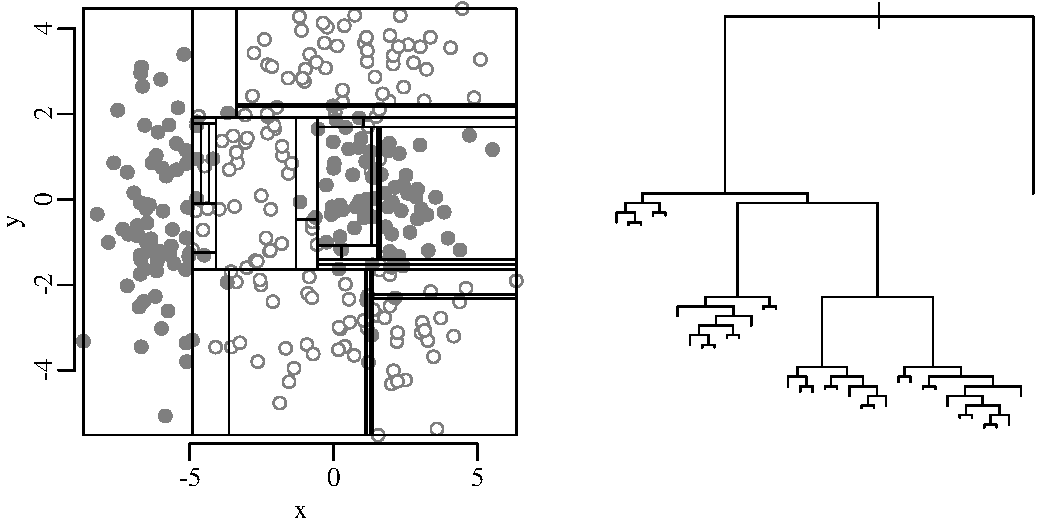
\includegraphics[width=\textwidth]{../figures/overfittedCARTscatter.pdf}\\
\end{minipage}
\begin{minipage}[t][][t]{.3\textwidth}
  \captionof{figure}{A recursive binary partition tree that perfectly
    classifies all the samples in Figure~\ref{fig:CARTdata}. The
    annotations of the dendrogram have been removed to reduce
    clutter. \\}
  \label{fig:overfittedCARTscatter}
\end{minipage}

The maximum sized tree thus obtained contains 35 terminal nodes and
perfectly describes the training data.  In other words, it has zero
\textbf{bias}.  However, for the purpose of prediction, this tree is
not optimal, because it overfits the training data, causing high
\textbf{variance}. One way to estimate the misclassification rate is
to use a separate set of test data whose affinities ($\circ$ or
$\bullet$) are known, but which were not used to train the decision
tree. Another method is \textbf{cross validation}. This method works
as follows:

\begin{enumerate}
\item divide the training data into ten equal parts;
\item\label{it:cv1} remove one of the parts, and use the remaining
  nine to create a decision tree;
\item\label{it:cv2} put the removed part in the tree and count the
  number of misclassified samples;
\item repeat steps~\ref{it:cv1} and \ref{it:cv2}, but this time
  removing the second fraction;
\item repeat until all ten parts have been assessed.
\end{enumerate}

The tree with optimal \textbf{predictive power} is smaller than the
largest possible tree, and can be found by `pruning' it. Define the
``cost-complexity criterion'' of a tree $T$ as

\begin{equation}
  \label{eq:cp}
  cp_{\alpha}(T) = \sum_{m=1}^{|T|} N_m Q_m + \alpha|T|
\end{equation}

\noindent where $|T|$ is the number of terminal nodes in the tree $T$,
$N_m$ the number of observations in the $m$\textsuperscript{th}
terminal node; $Q_m$ the impurity of the $m$\textsuperscript{th} node,
defined by Equation~\ref{eq:Q}; and $\alpha$ a tuning parameter.  For
a given $\alpha \geq 0$, it is possible to find the subtree
$T_{\alpha} \subset T_0$ that minimises $cp_{\alpha}(T)$ over all
possible subtrees of the largest possible tree $T_0$:

\begin{equation}
  \label{eq:Ta}
  T_{\alpha} = \underset{T \subset T_0}{\min} cp_{\alpha}(T)
\end{equation}

Repeating this procedure for a range of values $0 \leq \alpha <
\infty$ produces a finite nested sequence of trees
$\{T_0,T_{\alpha_1},...,T_{\alpha_{max}}\}$.  Except for $T_0$, these
trees no longer have only pure end-nodes. Impure end-nodes are
assigned to the class that dominates in them.  We then choose the
value $\alpha^*$ that minimises the cross validation error. For the
bivariate example dataset:

\noindent\begin{minipage}[t][][b]{.3\textwidth}
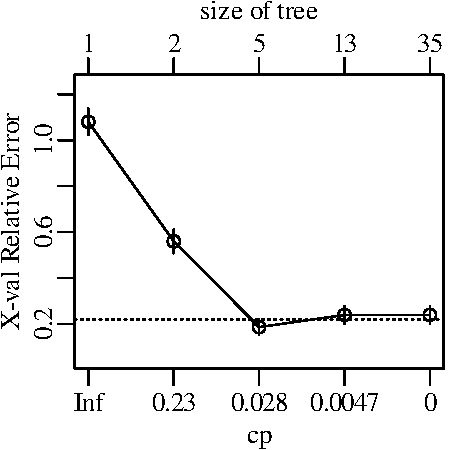
\includegraphics[width=\textwidth]{../figures/cvCART.pdf}\\
\end{minipage}
\begin{minipage}[t][][t]{.7\textwidth}
  \captionof{figure}{A plot of cross validated (CV) prediction error
    versus the number of nodes in the collection of nested subtrees
    shows a minimum at five splits.  The CV error of small trees is
    caused by bias, whereas the CV error of large tree is a result of
    variance.  There typically exist several trees with CV errors
    close to the minimum. Therefore, a `1-SE rule' is used, i.e.,
    choosing the smallest tree whose misclassification rate does not
    exceed the minimum CV error plus one standard error of the
    smallest CV error (dotted line).\\}
  \label{fig:cvCART}
\end{minipage}

For the bivariate example, this procedure generates a tree with four
splits and five terminal nodes:

\noindent\begin{minipage}[t][][b]{.7\textwidth}
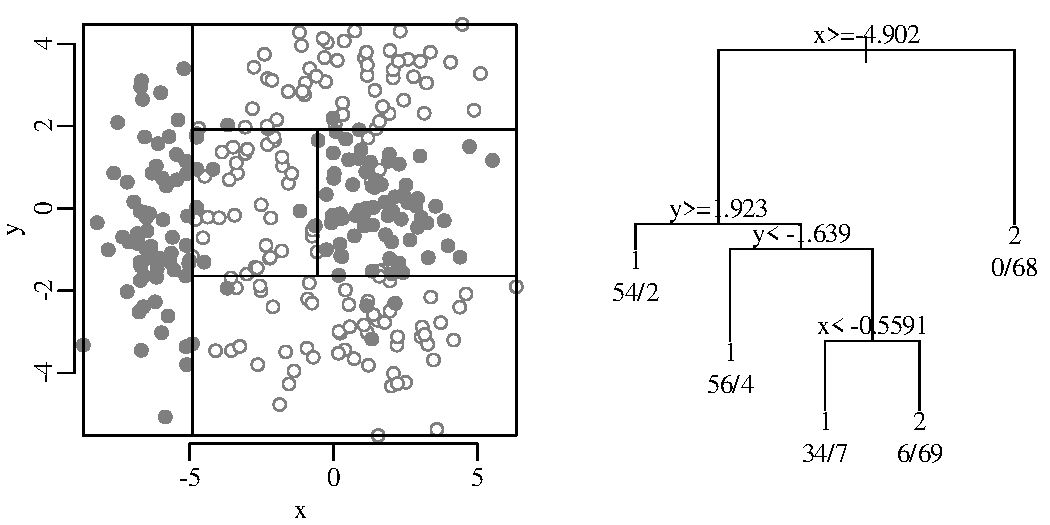
\includegraphics[width=\textwidth]{../figures/optimalCART.pdf}\\
\end{minipage}
\begin{minipage}[t][][t]{.3\textwidth}
  \captionof{figure}{The optimal tree for the bivariate test data.
    This tree misclassifies 19 of the 300 samples in the training data
    (6.3\%). The 10-fold cross validation error is 18\%.\\}
  \label{fig:optimalCART}
\end{minipage}

Like the discriminant analysis of Section~\ref{sec:LDA}, also decision
trees can be applied to, and are most useful for, datasets that
comprise more than two dimensions. Applying the method to Fisher's
iris data:

\noindent\begin{minipage}[t][][b]{.3\textwidth}
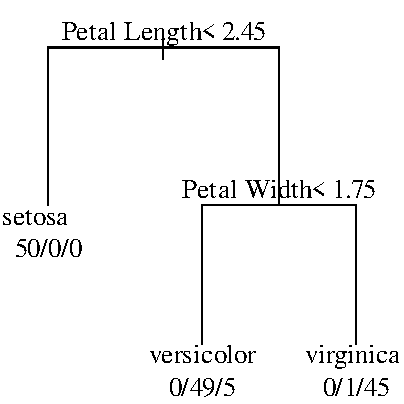
\includegraphics[width=\textwidth]{../figures/irisCART.pdf}\\
\end{minipage}
\begin{minipage}[t][][t]{.7\textwidth}
  \captionof{figure}{The optimal tree for Fisher's iris data. There
    are four variables (instead of two for the previous example) and
    three classes (instead of two for the previous example).  The
    optimal tree misclassifies 6 of the 150 flowers in the training
    data (4\%). The 10-fold cross validation error is 6\%.\\}
  \label{fig:irisCART}
\end{minipage}

Suppose that we have a new flower with a sepal length of 6.0~cm, a
sepal width of 3.0~cm, a petal length of 5.0~cm and a petal width of
1.5~cm. To which species does the flower belong? The petal length of
the new flower is greater than the 2.45~cm cutoff of the first split
and its petal width is less than the 1.75~cm cutoff of the second
split. Therefore the flower ends up in second terminal node of the
tree, suggesting that it belongs to species \emph{versicolor}.  This
is the same conclusion as the LDA classification shown in
Figure~\ref{fig:LDAnewiris}.


